\documentclass[journal,12pt,onecolumn]{IEEEtran}
\usepackage{cite}
\usepackage{graphicx}
\usepackage{amsmath,amssymb,amsfonts,amsthm}
\usepackage{algorithmic}
\usepackage{textcomp}
\usepackage{xcolor}
\usepackage{txfonts}
\usepackage{listings}
\usepackage{enumitem}
\usepackage{mathtools}
\usepackage{gensymb}
\usepackage{comment}
\usepackage[breaklinks=true]{hyperref}
\usepackage{tkz-euclide} 
\usepackage{caption}
\usepackage{listings}
\usepackage{gvv}                                        
\usepackage[latin1]{inputenc} 
\usetikzlibrary{arrows.meta, positioning}
\usepackage{xparse}
\usepackage{color}                                            
\usepackage{array}                                            
\usepackage{longtable}                                       
\usepackage{calc}                                             
\usepackage{multirow}
\usepackage{multicol}
\usepackage{hhline}                                           
\usepackage{ifthen}                                           
\usepackage{lscape}
\usepackage{tabularx}
\usepackage{array}
\usepackage{float}
\newtheorem{theorem}{Theorem}[section]
\newtheorem{problem}{Problem}
\newtheorem{proposition}{Proposition}[section]
\newtheorem{lemma}{Lemma}[section]
\newtheorem{corollary}[theorem]{Corollary}
\newtheorem{example}{Example}[section]
\newtheorem{definition}[problem]{Definition}
\newcommand{\BEQA}{\begin{eqnarray}}
\newcommand{\EEQA}{\end{eqnarray}}
\usepackage{float}
\theoremstyle{remark}
\usepackage{circuitikz}
\usepackage{tikz}\title{}
\title{\Huge MN:MINING ENGINEERING}
\author{Vaishnavi Ramkrishna Anantheertha-EE25BTECH11059}
\begin{document}
\maketitle

\section*{Q.1--Q.5 carry one mark each}
\begin{enumerate}
\item Mr. X speaks \_\_\_\_\_\_ Japanese \_\_\_\_\_\_ Chinese.  

\hfill\brak{GATE\ MN\ 2022}
\begin{multicols}{4}
\begin{enumerate}
\item neither / or 
\item either / nor
\item neither / nor
\item also / but
\end{enumerate}
\end{multicols}
\item A sum of money is to be distributed among $P, Q, R,$ and $S$ in the proportion $5 \colon 2 \colon 4 \colon 3$, respectively.  

If $R$ gets $\, 1000$ more than $S$, what is the share of $Q$ ?

\hfill\brak{GATE\ MN\ 2022}
\begin{multicols}{4}
\begin{enumerate}
\item $500$
\item $1000$
\item $1500$
\item $2000$
\end{enumerate}
\end{multicols}
\item A trapezium has vertices marked as $P, Q, R,$ and $S$ (in that order anticlockwise).  
The side $PQ$ is parallel to side $SR$.  

Further, it is given that $PQ = 11 \,\text{cm}, \; QR = 4 \,\text{cm}, \; RS = 6 \,\text{cm}, \; SP = 3 \,\text{cm}$.  

What is the shortest distance between $PQ$ and $SR$ (in cm)?

\hfill\brak{GATE\ MN\ 2022}    
\begin{enumerate}
    \item $1.80$
    \item $2.40$
    \item $4.20$
    \item $5.76$

\end{enumerate}
\item The figure shows a grid formed by a collection of unit squares. The unshaded unit square in the grid represents a hole.
\begin{figure}[H]
  \centering
  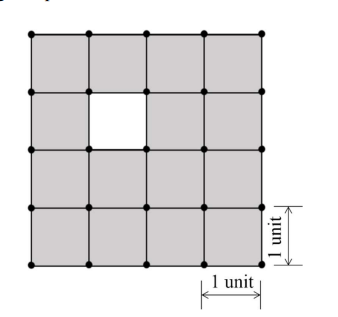
\includegraphics[width=0.4\columnwidth]{figs/grid.png}
  \caption{Grid}
  \label{fig:grid}
\end{figure}
What is the maximum number of squares without a hole in the interior that
can be formed within the $4 \times 4$ grid using the unit squares as building blocks?

\hfill\brak{GATE\ MN\ 2022}
\begin{multicols}{4}
\begin{enumerate}
\item $15$
\item $20$ 
\item $21$
\item $26$
\end{enumerate}
\end{multicols}
\item An art gallery engages a security guard to ensure that the items displayed are
protected. The diagram below represents the plan of the gallery where the
boundary walls are opaque. The location the security guard posted is identified
such that all the inner space (shaded region in the plan) of the gallery is within
the line of sight of the security guard.
If the security guard does not move around the posted location and has a $360^\circ$ view, which one of the following correctly represents the set of ALL possible
locations among the locations P, Q, R and S, where the security guard can be
posted to watch over the entire inner space of the gallery. 
\begin{figure}[H]
  \centering
  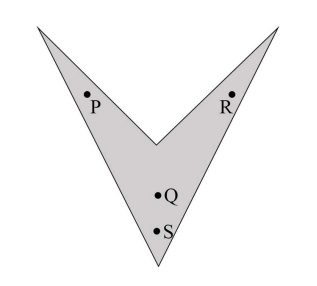
\includegraphics[width=0.4\columnwidth]{figs/tri.png}
  \caption{diagram}
  \label{fig:tri}
\end{figure}
\hfill\brak{GATE\ MN\ 2022} 
\begin{multicols}{4}
\begin{enumerate}
\item P and Q 
\item Q 
\item Q and S
\item R and S 
\end{enumerate}
\end{multicols}
\item Mosquitoes pose a threat to human health. Controlling mosquitoes using chemicals may have undesired consequences. In Florida, authorities have used
genetically modified mosquitoes to control the overall mosquito population. It remains to be seen if this novel approach has unforeseen consequences.
Which one of the following is the correct logical inference based on the information in the above passage? 

\hfill\brak{GATE\ MN\ 2022}
\begin{enumerate}
\item Using chemicals to kill mosquitoes is better than using genetically modified mosquitoes because genetic engineering is dangerous 
\item Using genetically modified mosquitoes is better than using chemicals to kill mosquitoes because they do not have any side effects 
\item Both using genetically modified mosquitoes and chemicals have undesired consequences and can be dangerous 
\item Using chemicals to kill mosquitoes may have undesired consequences but it is not clear if using genetically modified mosquitoes has any negative
consequence 
\end{enumerate}

\item  Consider the following inequalities:  

\begin{enumerate}
    \item[(i)] $2x - 1 \geq 7$
    \item[(ii)] $2x - 9 \leq 1$
\end{enumerate}

Which one of the following expressions satisfies the above two inequalities?    

\hfill\brak{GATE\ MN\ 2022}
\begin{multicols}{4}
\begin{enumerate}
\item $x \leq -4$
\item $-4 \leq x \leq 4$ 
\item $4 \leq x \leq 5$
\item $x \geq 5$
\end{enumerate}
\end{multicols}
\item Four points P\brak{0,1}, Q\brak{0,-3}, R\brak{-2,-1}, and S\brak{2,-1} represent the vertices
of a quadrilateral.
What is the area enclosed by the quadrilateral? 

\hfill\brak{GATE\ MN\ 2022}
\begin{multicols}{4}
\begin{enumerate}
\item $4$
\item $4\sqrt{2}$ 
\item $8$
\item $8\sqrt{2}$
\end{enumerate}
\end{multicols}
\item In a class of five students P, Q, R, S and T, only one student is known to have copied in the exam. The disciplinary committee has investigated the situation
and recorded the statements from the students as given below. 
\textbf{Statement of P:} R has copied in the exam.  

\textbf{Statement of Q:} S has copied in the exam.  

\textbf{Statement of R:} P did not copy in the exam.  

\textbf{Statement of S:} Only one of us is telling the truth.  

\textbf{Statement of T:} R is telling the truth.  

The investigating team had authentic information that $S$ never lies.  

Based on the information given above, the person who has copied in the exam is \_\_\_\_\_\_. 

\hfill\brak{GATE\ MN\ 2022}
\begin{multicols}{2}
\begin{enumerate}
    \item R
    \item P
    \item Q
    \item T
\end{enumerate}
\end{multicols}
\item Consider the following square with the four corners and the center marked as $P, Q, R, S$ and $T$ respectively.  

Let $X, Y,$ and $Z$ represent the following operations:  

\begin{itemize}
    \item $X$: rotation of the square by $180^\circ$ with respect to the $S$-$Q$ axis.  
    \item $Y$: rotation of the square by $180^\circ$ with respect to the $P$-$R$ axis.  
    \item $Z$: rotation of the square by $90^\circ$ clockwise with respect to the axis perpendicular, going into the screen and passing through the point $T$.  
\end{itemize}

Consider the following three distinct sequences of operation (which are applied in the left to right order): 
\begin{enumerate}
    \item $XYZZ$
    \item $XY$
    \item $ZZZZ$
\end{enumerate}

Which one of the following statements is correct as per the information provided above?  

\hfill\brak{GATE\ MN\ 2022}
\begin{multicols}{2}
\begin{enumerate}
\item The sequence of operations (1) and (2) are equivalent
\item The sequence of operations (1) and (3) are equivalent 
\item The sequence of operations (2) and (3) are equivalent
\item The sequence of operations (1), (2) and (3) are equivalent 
\end{enumerate}
\end{multicols}
\item The value of $\lim_{x \to 0} \frac{(1-x)^n - 1}{x}$ is 

\hfill\brak{GATE\ MN\ 2022}
\begin{multicols}{4}
\begin{enumerate}
\item $0$
\item $1$
\item $-n$
\item $n$
\end{enumerate}
\end{multicols}
\item A velocity field in Cartesian coordinate system is expressed as  

\[
\mathbf{v} = x \hat{i} + y \hat{j} + p(z)\hat{k}, \quad \text{where } p(0) = 0
\]  
If $\nabla \cdot \mathbf{v} = 0$, $p(z)$ is

\hfill\brak{GATE\ MN\ 2022}
\begin{multicols}{2}
\begin{enumerate}
\item $0$
\item $-2z$
\item $2$
\item $2z$
\end{enumerate}
\end{multicols}
\item The constant term of the Fourier coefficients of the periodic function  

\[
f(x) = 
\begin{cases}
 -k, & -\pi < x < 0 \\[6pt]
 \;\;k, & 0 < x < \pi
\end{cases}, 
\quad f(x+2\pi) = f(x), \quad k = \text{constant}
\]

is  

\hfill\brak{GATE\ MN\ 2022}
\begin{multicols}{2}
\begin{enumerate}
  \item $k$
  \item $2k$
  \item $2\pi$
  \item $0$
\end{enumerate}
\end{multicols}

 \item Two vectors x and y are shown in the figure. The projection vector of x on y is
 \begin{figure}[H]
  \centering
  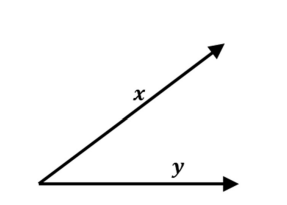
\includegraphics[width=0.4\columnwidth]{figs/vec.png}
  \caption{Vectors}
  \label{fig:vec}
\end{figure}
\hfill\brak{GATE\ MN\ 2022}
\begin{multicols}{4}
\begin{enumerate}
\item $\dfrac{x^T y}{y^T y} \, y$
\item $x \times y$
\item $\dfrac{x \times y}{y^T y}$
\item $\dfrac{x^T y}{x^T x} \, x$
\end{enumerate}
\end{multicols}

\item A deposit has the grade attribute $X \in [0,30]$ with a density function $f(x)$.  
For a cut-off grade $x_c$, the proportion of the ore in the deposit is given by 

\hfill\brak{GATE\ MN\ 2022}
\begin{multicols}{2}
\begin{enumerate}
    \item $\int_{0}^{30} f(x)\,dx - \int_{0}^{x_c} f(x)\,dx$
    \item $\dfrac{1}{2} \int_{0}^{30} f(x)\,dx - \int_{0}^{x_c} f(x)\,dx$
    \item $\dfrac{1}{2} \int_{0}^{30} f(x)\,dx + \int_{0}^{x_c} f(x)\,dx$
    \item $\int_{0}^{x_c} f(x)\,dx$
\end{enumerate}
\end{multicols}

\item The drilling technique applicable for mineral exploration is 

\hfill\brak{GATE\ MN\ 2022}
\begin{multicols}{2}
\begin{enumerate}
\item Percussive drilling 
\item Tricone roller drilling 
\item Rotary-percussive drilling
\item Diamond core drilling 
\end{enumerate}
\end{multicols}
\item Match the rock with its metamorphosed form

\hfill\brak{GATE\ MN\ 2022}
\begin{table}[H]
  \centering
  \caption{Match The Following}
  \begin{tabular}{>{\bfseries}l l}
Specification & Outer Diameter in mm \\
P. AW & p. 34.9 \\
Q. BW & q. 44.4 \\
R. EW & r. 54.0 \\
S. NW & s. 66.7 \\
\end{tabular}


  \label{tab:Table1}
\end{table}
\begin{multicols}{2}
\begin{enumerate}
\item P-II, Q-IV, R-I, S-III 
\item P-III, Q-I, R-IV, S-II
\item P-IV, Q-III, R-I, S-II
\item P-II, Q-III, R-IV, S-I 
\end{enumerate}
\end{multicols}

\item Identify the WRONG statement:
Break-even stripping ratio 

\hfill\brak{GATE\ MN\ 2022}
\begin{enumerate}
\item takes into account the maximum pit slope that is safe  
\item helps in determining the volume of the overburden  
\item presents the maximum possible mine size that is economical 
\item takes into account the life of the mine
\end{enumerate}

\item A square pattern of blasting is shown in the figure. For the case of simultaneous blast, identify the zone of no fragmentation
\begin{figure}[H]
\centering
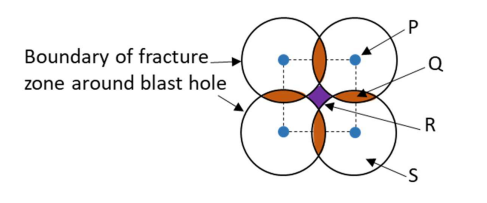
\includegraphics[width=0.4\columnwidth]{figs/blasting.png}
\caption{Blasting}
\label{fig:blast}
\end{figure}
\hfill\brak{GATE\ MN\ 2022}
\begin{multicols}{4}
\begin{enumerate}
\item P
\item Q
\item R
\item S
\end{enumerate}
\end{multicols}
\item In the truss shown in the figure, the force in the member BD, in kN is
\begin{figure}[H]
\centering
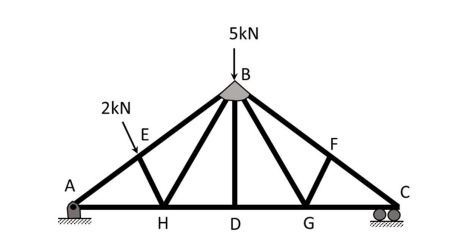
\includegraphics[width=0.4\columnwidth]{figs/truss1.png}
\caption{Diagram}
\label{fig:t}
\end{figure}

\hfill\brak{GATE\ MN\ 2022}

\begin{multicols}{4}
\begin{enumerate}
\item $7$
\item $5$
\item $2$
\item $0$
\end{enumerate}
\end{multicols}
\item The correct vertical stress profile in the case of tributary area method for pillar
design is 
\begin{figure}[H]
\centering
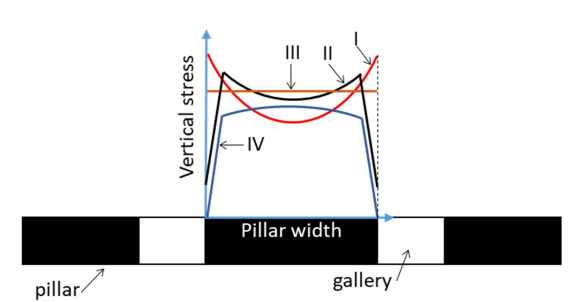
\includegraphics[width=0.4\columnwidth]{figs/pillar.png}
\caption{Diagram}
\label{fig:p}
\end{figure}

\hfill\brak{GATE\ MN\ 2022}
\begin{multicols}{4}
\begin{enumerate}
\item $I$
\item $II$
\item $III$
\item $IV$
\end{enumerate}
\end{multicols}
\item The bottom section of a stoping block has dimensions $200 m\times40 m$. If the modified RMR of rock mass is $50$, the appropriate method of mining on the basis of Laubscher chart in the figure is 
\begin{figure}[H]
\centering
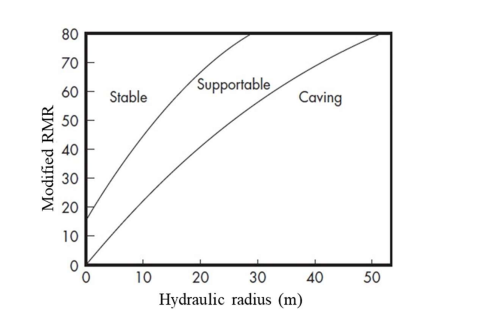
\includegraphics[width=0.4\columnwidth]{figs/RMR.png}
\caption{Diagram}
\label{fig:RMR}
\end{figure}

\hfill\brak{GATE\ MN\ 2022}
\begin{multicols}{4}
\begin{enumerate}
\item Shrinkage stoping
\item Cut and fill 
\item Block Caving
\item Sublevel stoping
\end{enumerate}
\end{multicols}

\item Match the machine with its component.
\begin{table}[H]
  \centering
  \caption{Match The Following}
  \begin{center}
\begin{tabular}{|c|c|c|c|c|c|}
\hline
Mass of particles, g      & 2   & 5   & 7   & 4   & 1    \\
\hline
Mean size of particles, $\mu$m & 350 & 240 & 200 & 150 & 100 \\
\hline
\end{tabular}
\end{center}
  \label{tab:table2}
\end{table}
\hfill\brak{GATE\ MN\ 2022}
\begin{multicols}{2}
\begin{enumerate}
\item P-III, Q-IV, R-I, S-II  
\item P-IV, Q-III, R-I, S-II  
\item P-III, Q-IV, R-II, S-I 
\item P-IV, Q-III, R-II, S-I 
\end{enumerate}
\end{multicols}
\item Which one of the following is NOT a notifiable disease as per Indian mining legislation?

\hfill\brak{GATE\ MN\ 2022}
\begin{multicols}{2}
\begin{enumerate}
\item Silicosis
\item Noise induced hearing loss
\item Nystagmus 
\item Asbestosis 
\end{enumerate}
\end{multicols}

\item If the ambient lapse rate is higher than the dry adiabatic lapse rate, the atmosphere is 

\hfill\brak{GATE\ MN\ 2022}
\begin{multicols}{4}
\begin{enumerate}
\item stable
\item neutral 
\item unstable 
\item strongly stable
\end{enumerate}
\end{multicols}

\item Identify the WRONG statement:
The application of controlled air recirculation in an underground work place can

\hfill\brak{GATE\ MN\ 2022}
\begin{enumerate}
\item increase the air velocity at the work place 
\item lead to increased concentration of contaminants in the work place
\item require the installation of an additional fan in the system
\item lead to overall ventilation cost savings
\end{enumerate}
\item The correct order of pavement layers for a haul road from top to bottom is 

\hfill\brak{GATE\ MN\ 2022}
\begin{enumerate}
\item  Wearing course $\rightarrow$ Base $\rightarrow$ Sub base $\rightarrow$ Sub grade
\item Wearing course $\rightarrow$ Sub base $\rightarrow$ Base $\rightarrow$ Sub grade
\item Wearing course $\rightarrow$ Sub grade $\rightarrow$ Sub base $\rightarrow$ Base
\item Wearing course $\rightarrow$ Base $\rightarrow$ Sub grade $\rightarrow$ Sub base
\end{enumerate}
\item A mining company produces iron ore and sells to another company. Royalty to be paid is on the basis of 

\hfill\brak{GATE\ MN\ 2022}
\begin{multicols}{2}
\begin{enumerate}
\item quantity of ore produced 
\item quantity of ore sold 
\item difference between the quantities of ore produced and sold
\item net profit 
\end{enumerate}
\end{multicols}

\item The cost of a screw compressor with an estimated life of $15$ years is $21,00,000$. If the depreciation of the compressor charged, using sum-of-the-years-digits
method, at the end of 4th year is $2,00,000,$ the salvage value, is.(round off to one decimal place) 

\hfill\brak{GATE\ MN\ 2022}
\item A safety device consists of two independent critical components x1 and x2.The failure of any one or both of these components can cause an accident.The failure probabilities of components x1 and x2 are $0.2$ and $0.1$, respectively.The probability of occurrence of an accident is 

\hfill\brak{GATE\ MN\ 2022}
\item In a levelling survey, a reading is taken as $2.25$ m. However, along the line of sight there is deflection of $20$ cm with respect to vertical position of the staff. The correct reading, in m is. (round off to two decimal places) 

\hfill\brak{GATE\ MN\ 2022}

\item Water flows through a vertical sand column of cross sectional area $4000 \; \text{mm}^2$ and length $300 \; \text{mm}$. For a water head of $600 \; \text{mm}$, quantity of seepage water is $100 \; \text{mm}^3/\text{min}$. The hydraulic conductivity of the sand column, in $\text{mm}/\text{min}$ is (round off to three decimal places).

\hfill\brak{GATE\ MN\ 2022}
\item The modified Lauffer diagram as shown in the figure relates to roof span, RMR and stand-up time. In a metal mine, roof span of a drive is $4 m$. If the RMR of the rock mass changes from $40$ to $60$, then the stand-up time increases by a factor of.     (round off to two decimal places) 
\begin{figure}[H]
\centering
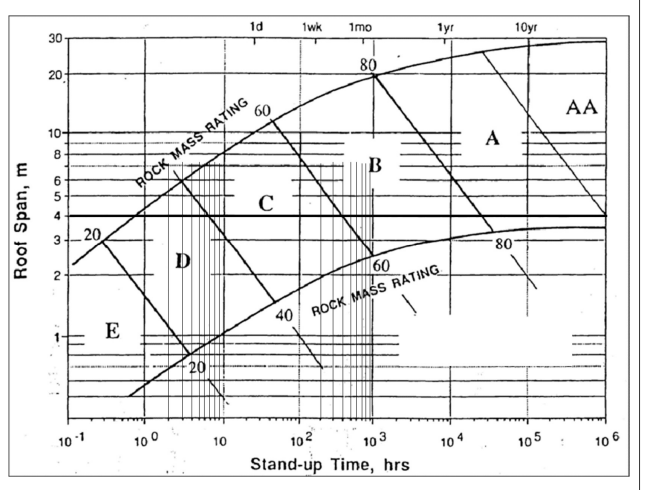
\includegraphics[width=0.4\columnwidth]{figs/gRMR.png}
\caption{Diagram}
\label{fig:gRMR}
\end{figure}

\hfill\brak{GATE\ MN\ 2022}
\item In a friction winder, the skip accelerates to a steady speed over a time span of $15$ s from the start. The torque vs. time diagram for the winding cycle is shown in the figure. The deceleration time in seconds is      (round off to one decimal place)
\begin{figure}[H]
\centering
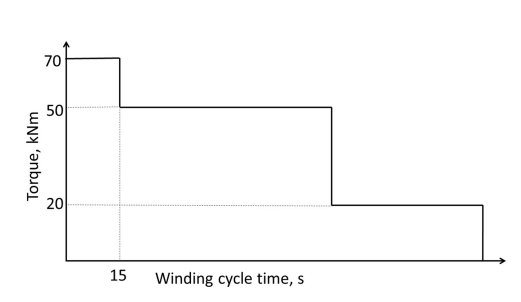
\includegraphics[width=0.4\columnwidth]{figs/friction.png}
\caption{Diagram}
\label{fig:fric}
\end{figure}

\hfill\brak{GATE\ MN\ 2022}
\item At a measurement station, the air quality parameters PM$_{2.5}$, NO$_2$ and O$_3$ 
have the AQI sub-index values as 180, 96, and 84, respectively. 
The AQI for the station is \underline{\hspace{1.5cm}}. 
\textit{(in integer)}

\hfill\brak{GATE\ MN\ 2022}
\item Match The following 
\begin{table}[H]
  \centering
  \caption{Match The Following}
  \begin{table}[ht]
\centering
\begin{tabular}{|l|l|}
\hline
\textbf{Column I} & \textbf{Column II} \\ \hline
P. Hydraulic Conductivity   & 1. Upper limit of moisture available to plant \\ \hline
Q. Permeability            & 2. All soil pores are filled with water         \\ \hline
R. Viscosity               & 3. Soil capillarity                            \\ \hline
S. Surface Tension         & 4. Properties of fluid as well as soil          \\ \hline
T. Saturation Capacity     & 5. Property of the medium                      \\ \hline
U. Field Capacity          & 6. Internal friction that brings about resistance to flow \\ \hline
\end{tabular}
\end{table}
  \label{tab:table3}
\end{table}
\hfill\brak{GATE\ MN\ 2022}
\begin{multicols}{2}
\begin{enumerate}
\item P $\to$ II,\; Q $\to$ III,\; R $\to$ I,\; S $\to$ II
\item P $\to$ III,\; Q $\to$ IV,\; R $\to$ I,\; S $\to$ II
\item P $\to$ II,\; Q $\to$ I,\; R $\to$ IV,\; S $\to$ III
\item P $\to$ III,\; Q $\to$ IV,\; R $\to$ II,\; S $\to$ I
\end{enumerate}
\end{multicols}

\item The closest match of the scatter plot between the variables X and Y with the approximate attribute is 

\hfill\brak{GATE\ MN\ 2022}
\begin{figure}[H]
  \centering
  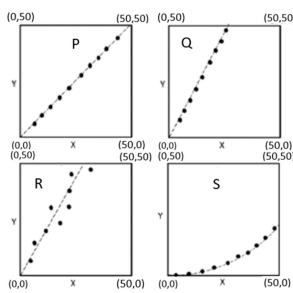
\includegraphics[width=0.4\columnwidth]{figs/SG.png}
  \caption{GRAPH}
  \label{fig:SG}
\end{figure}
\begin{table}[H]
  \centering
  \caption{Match The Following}
  \begin{center}
\begin{tabular}{|c|c|c|c|c|c|c|}
\hline
\textbf{S. No.} & 1 & 2 & 3 & 4 & 5 & 6 \\
\hline
\textbf{H/W (mm/kg)} & 23.9 & 23.7 & 21.3 & 22.1 & 25.3 & 23.3 \\
\hline
\end{tabular}
\end{center}
  \label{tab:table4}
\end{table}
\vspace{1em}

$\sigma_x =$ standard deviation of variable X \\
$\sigma_y =$ standard deviation of variable Y \\
$\rho_{xy} =$ Pearson's correlation coefficient between X and Y
\begin{multicols}{2}
\begin{enumerate}
\item P $\to$ II,\; Q $\to$ III,\; R $\to$ I,\; S $\to$ II
\item P $\to$ III,\; Q $\to$ IV,\; R $\to$ I,\; S $\to$ II
\item P $\to$ II,\; Q $\to$ I,\; R $\to$ IV,\; S $\to$ III
\item P $\to$ III,\; Q $\to$ IV,\; R $\to$ II,\; S $\to$ I
\end{enumerate}
\end{multicols}

\item A $3$-point borehole extensometer is installed to identify the location of a single discontinuity plane in a hanging wall rock by measuring deformations at three
locations as shown in the figure. The absolute readings of deformations measured on two different dates are listed in the table. Based on the measured data the most
likely inference is 
\begin{figure}[H]
  \centering
  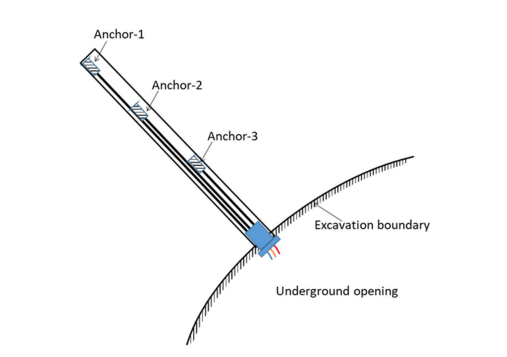
\includegraphics[width=0.4\columnwidth]{figs/anchor.png}
  \caption{Diagram}
  \label{fig:anc}
\end{figure}
\begin{table}[H]
  \centering
  \caption{Match The Following}
  \begin{center}
\begin{tabular}{|l|c|c|}
\hline
Description & \textbf{P} & \textbf{Q} \\
\hline
R.L. of the ground surface, m & 220 & 220 \\
Depth of piezometer, m & 60 & 50 \\
Depth to groundwater level from ground surface, m & 60 & 50 \\
\hline
\end{tabular}
\end{center}
  \label{tab:table5}
\end{table}
\hfill\brak{GATE\ MN\ 2022}

\begin{enumerate}
\item Discontinuity between Anchor-1 and Anchor-2 
\item Discontinuity between Anchor-2 and Anchor-3 
\item Discontinuity between Anchor-3 and excavation boundary
\item No noticeable discontinuity
\end{enumerate}
\item From a coal seam of a mine $1000$ tonnes of coal is produced per day. The seam has inflammable gas emission rate of $14000$ $m^{3}$ per day. Percentage of inflammable gas in general body of air is $0.14$. The gassiness of the seam is

\hfill\brak{GATE\ MN\ 2022}
\begin{multicols}{4}
\begin{enumerate}
\item Degree IV
\item Degree III
\item Degree II
\item Degree I
\end{enumerate}
\end{multicols}

\item Match the semi-variogram shape with the model name and the property
\begin{figure}[H]
  \centering
  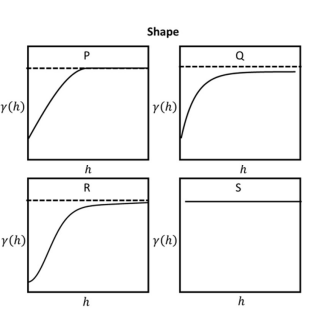
\includegraphics[width=0.4\columnwidth]{figs/semi.png}
  \caption{Diagram}
  \label{fig:sem}
\end{figure}
\begin{table}[H]
  \centering
  \caption{Match The Following}
  \begin{table}[h!]
\centering
\begin{tabular}{|c|c|c|c|c|c|c|c|}
\hline
\textbf{Contour Value (m)} & 100 & 101 & 102 & 103 & 104 & 105 & 106 \\
\hline
\textbf{Area Enclosed (m$^2$)} & 440 & 580 & 640 & 740 & 960 & 1100 & 1240 \\
\hline
\end{tabular}
\end{table}
  \label{tab:table6}
\end{table}
\hfill\brak{GATE\ MN\ 2022}

\begin{enumerate}
\item $P\to \mathrm{III}\to E,\quad Q\to \mathrm{II}\to F,\quad R\to \mathrm{IV}\to E,\quad S\to \mathrm{I}\to G$
\item $P\to \mathrm{II}\to F,\quad Q\to \mathrm{I}\to G,\quad R\to \mathrm{III}\to E,\quad S\to \mathrm{IV}\to E$
\item $P\to \mathrm{IV}\to G,\quad Q\to \mathrm{III}\to F,\quad R\to \mathrm{II}\to E,\quad S\to \mathrm{I}\to E$
\item $P\to \mathrm{II}\to E,\quad Q\to \mathrm{I}\to E,\quad R\to \mathrm{III}\to F,\quad S\to \mathrm{IV}\to G$
\end{enumerate}

\item In a uniaxial compressive strength test, a rock sample of diameter $50 \ \text{mm}$ fails at an angle of $60^\circ$. If the peak load at failure is $120 \ \text{kN}$, the normal and shear stresses 
on the failure plane respectively, in MPa are \underline{\hspace{1.5cm}} and \underline{\hspace{1.5cm}}.
\begin{figure}[H]
  \centering
  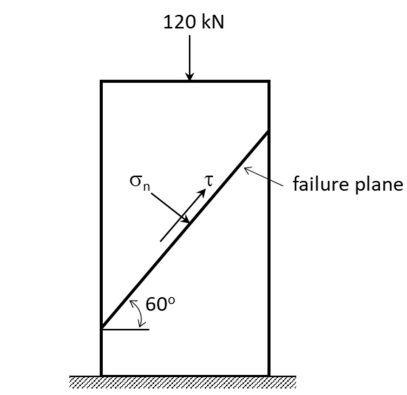
\includegraphics[width=0.4\columnwidth]{figs/stress.png}
  \caption{Diagram}
  \label{fig:ste}
\end{figure}
\begin{table}[H]
  \centering
  \caption{Match The Following}
  \begin{center}
\renewcommand{\arraystretch}{1.5}
\begin{tabular}{|c|c|c|c|}
\hline
\textbf{Temperature ($^\circ$C)} & 30 & 45 & 65 \\ \hline
\textbf{Saturation Vapour Pressure (kPa)} & 4.16 & 9.48 & 24.92 \\ \hline
\textbf{Latent Heat of Vapourisation (kJ kg$^{-1}$)} & 2430.7 & 2394.9 & 2346.3 \\ \hline
\end{tabular}
\end{center}
  \label{tab:table7}
\end{table}

\hfill\brak{GATE\ MN\ 2022}
\begin{multicols}{4}
\begin{enumerate}
\item $20, 15$
\item $0, 30$
\item $0, 31$
\item $40, 0$
\end{enumerate}
\end{multicols}

\item Let $f(x)$ be a continuous and differentiable function on $[3,18]$. 
If $f(3) = -50$ and $f'(x) \leq 20$, then the largest possible value of $f(18)$ is \_\_\_\_\_. (in integer)
\hfill\brak{GATE\ MN\ 2022}

\item  Let $\dfrac{dT}{dt} \propto (T_R - T)$, where $T_R$ and $T$ are temperatures in degree centigrade of a room and thermometer, respectively, and $t$ denotes time in minutes. 
A thermometer at a reading of $2^{\circ}C$ is brought in a room of temperature $40^{\circ}C$. 
Two minutes later, the thermometer reads $15^{\circ}C$. 
The time elapsed in minutes when the thermometer reads $39.5^{\circ}C$, is \_\_\_\_\_. 
(\textit{round off to two decimal places})

\hfill\brak{GATE\ MN\ 2022}
\item A project network comprises five activities as shown below. The activity durations, in days, are as
indicated. Crashing of any activity costs Rs.$1000$ per day. If the project is crashed to the shortest possible duration, the total crashing cost in Rupees is

\hfill\brak{GATE\ MN\ 2022}
\item In a health centre, the probability of full occupancy of COVID beds for a day is $0.8$. Assuming Binomial probability distribution, the probability of full occupancy exactly for $5$ days in a week, is\_\_\_. (round off to three decimal places) 

\hfill\brak{GATE\ MN\ 2022}
\item Following information is given for a drilling operation to be carried out for 
overburden removal in a surface mine. 
\begin{table}[H]
  \centering
  \caption{Match The Following}
  \input{Tables/Table8}
  \label{tab:table8}
\end{table}

The amount of explosive per unit length of charge in kg/m, is \_\_\_\_\_. 
(\textit{round off to two decimal places})

\hfill\brak{GATE\ MN\ 2022}
\item The shaft-top coordinates of two vertical shafts are given below. The depth of the shaft A and B are $200 m$ and $149 m$, respectively.
\begin{table}[H]
  \centering
  \caption{Match The Following}
  \input{Tables/Table9}
  \label{tab:table9}
\end{table}

\hfill\brak{GATE\ MN\ 2022}
\item The downward gradient of the line joining the bottom of the two shafts in degrees, is \_\_\_\_\_. 
(\textit{round off to two decimal places}) \\[2em]


The oxygen-balanced equation for explosive ANFO is given below.  

\[
3NH_4NO_3 + CH_2 \;\; \rightarrow \;\; 7H_2O + CO_2 + 3N_2
\]

For $100 \, \text{litre}$ of fuel oil having density $850 \, \text{kg/m}^3$, the amount of ammonium nitrate 
to be mixed, in kg, is \_\_\_\_\_. \\
(\textit{round off to two decimal places})


\hfill\brak{GATE\ MN\ 2022}
\item Two weightless cables of equal length and cross sectional area are hanging from a
ceiling as shown in the figure. They are connected by a horizontal light bar of length 1.0 m and pulled by a force, F. The modulus of elasticity of Cable-1 and Cable-2 are 50 GPa and 200 GPa, respectively. If the deformation in both the cables is equal,the distance, in m is. (round off to one decimal place) 
\begin{figure}[H]
  \centering
  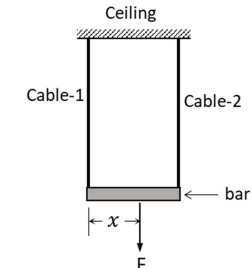
\includegraphics[width=0.2\columnwidth]{figs/cab.png}
  \caption{diagram}
  \label{fig:4849}
\end{figure}
\item A circular tunnel of radius $3$ m is constructed in a hydrostatic stress field of $15$ MPa.The modulus of elasticity and Poissons ratio of the rock are $5$ GPa and $0.25$, respectively. A uniform support pressure p is applied at tunnel boundary to restrict
the radial deformation at the tunnel boundary to $4$ mm. The value of p in MPa is. (round off to two decimal places) 

\hfill\brak{GATE\ MN\ 2022}
\item The extraction ratio during development of a bord and pillar panel is $0.15$ in a flat coal seam. The panel is further extracted by widening the galleries, and the extraction ratio changes to $0.25$. The percentage change in pillar stress, considering tributary area method, is. (round off to two decimal places) 

\hfill\brak{GATE\ MN\ 2022}
\item  In a small metal mine a battery powered locomotive hauls a train of mine tubs 
such that:  

\begin{itemize}
    \item The weight of the train of mine tubs, tonne : $3.0$
    \item The coefficient of friction between the wheels and the rails : $0.06$
    \item The coefficient of adhesion between the loco wheels and the rails : $0.2$
    \item Time required from the start to reach speed of $1.8 \ \text{m/s}$ through constant acceleration, min : $3.0$
    \item Upward gradient to be negotiated : $1 \text{ in } 20$
\end{itemize}

The minimum weight of the locomotive in tonnes to meet these design requirements, is \underline{\hspace{2cm}}.  
\textit{(round off to one decimal place)}

\hfill\brak{GATE\ MN\ 2022}
\item  In a surface mine bench, overburden is removed by the shovel--dumper combination.  
For the dumper:  

\begin{itemize}
    \item Time required at the loading station : $3.0 \ \text{min}$
    \item Time required at the unloading station : $1.0 \ \text{min}$
    \item Distance between loading and unloading stations : $4.5 \ \text{km}$
    \item Average speed during loaded travel : $12.0 \ \text{km/hr}$
    \item Average speed during empty travel : $18.0 \ \text{km/hr}$
\end{itemize}

Minimum number of dumpers required to avoid idle time of the shovel, is \underline{\hspace{1.5cm}}. \\
\textit{(in integer)}
\hfill\brak{GATE\ MN\ 2022}

\item In a bord and pillar development panel, headings of $4.4 \ \text{m} \times 2.5 \ \text{m}$ are advanced using solid blasting.  
The average pull per round of blast is $1.2 \ \text{m}$. On an average $12$ faces are blasted per day.  
Density of coal is $1500 \ \text{kg/m}^3$. The mine operates in three shifts.  

If the average daily employment is $330$ persons, labour productivity (OMS) of the panel in tonne, is \underline{\hspace{1.5cm}}.  
\textit{(round off to two decimal places)} 

\hfill\brak{GATE\ MN\ 2022}
\item In a longwall face, the full seam thickness of $3 \ \text{m}$ is cut by a shearer with a web of depth $0.7 \ \text{m}$.  
The hauling speed of shearer during cutting is $12 \ \text{m/min}$.  
The trough cross-section of AFC is $0.4 \ \text{m}^2$ and the average loading coefficient is $0.7$.  
In order to evacuate coal from the face without spillage, the speed of AFC, in m/s is \underline{\hspace{1.5cm}}.  
\textit{(round off to one decimal place)} 


\hfill\brak{GATE\ MN\ 2022}
\item A city is spread over an area of $20 \ \text{km} \times 40 \ \text{km}$.  
Wind, at an average speed of $4 \ \text{m/s}$, enters perpendicular to the $20 \ \text{km}$ long side.  
On a winter day the inversion layer exists over the city at a height of $100 \ \text{m}$.  
PM$_1$ is emitted from the city at a rate of $1 \ \text{kg/s}$.  

The steady state PM$_1$ concentration in the city air, in $\mu \text{g/m}^3$, assuming Box model, is \underline{\hspace{1.5cm}}.  
\textit{(round off to one decimal place)}  

\hfill\brak{GATE\ MN\ 2022}
\item  The point A as shown in the Coward flammability diagram represents the gas composition of a sealed-off area of a coal mine.  
The volume of the sealed-off area is $10000 \ \text{m}^3$.  
Inert gas is proposed to be injected into the sealed-off area so that the gas composition comes below the LEL (lower explosibility limit).  
The minimum volume of the inert gas required (at the same pressure as that of the sealed-off area), in $\text{m}^3$, is \underline{\hspace{1.5cm}}.  
\textit{(round off to one decimal place)}  


\hfill\brak{GATE\ MN\ 2022}
\item An underground workshop has dimensions of $8 \ \text{m}$ length, $6 \ \text{m}$ width and $4 \ \text{m}$ height.  
Four identical luminaires are placed at the four corners of the roof.  
Each luminaire is of $100 \ \text{W}$ capacity with luminous efficacy of $100 \ \text{lumen/W}$.  
Light is transmitted spherically from luminaires and there are no reflections.  
The illumination on the horizontal plane at the centre of the floor, in lux is \underline{\hspace{1.5cm}}.  
\textit{(round off to two decimal places)}  

\hfill\brak{GATE\ MN\ 2022}
\item An underground AC plant requires the delivery of $250 \ \text{US gpm}$ ($15.85 \ \text{US gpm} = 1.0 \ \text{lps}$) of chilled water.  
For this purpose, ice-pellets at $0^{\circ}\text{C}$ temperature (latent heat of melting, $334 \ \text{kJ/kg}$) are mixed with water at $20^{\circ}\text{C}$ (specific heat $4.18 \ \text{kJ/kg}^{\circ}\text{C}$) on the surface.  
The mixture is adiabatically transported to the underground location such that the water at $7^{\circ}\text{C}$ becomes available for the AC plant.  

The requirement of ice-pellets in tonne/hr to meet the design condition, is \underline{\hspace{1.5cm}}.  
\textit{(round off to two decimal places)} 


\hfill\brak{GATE\ MN\ 2022}
\item An intake shaft has resistance of $0.05 \ \text{Ns}^2/\text{m}^8$ up to a depth of $400 \ \text{m}$.  
The airflow rate is $100 \ \text{m}^3/\text{s}$ and the average density is $1.2 \ \text{kg/m}^3$.  
A barometer reads $99.375 \ \text{kPa}$ when placed on surface.  
Considering acceleration due to gravity is $9.81 \ \text{m/s}^2$, the reading of the barometer at the depth of $400 \ \text{m}$, in kPa is \underline{\hspace{1.5cm}}.  
\textit{(round off to two decimal places)}  



\hfill\brak{GATE\ MN\ 2022}

\item The net present values (NPV) of two mining project proposals A and B are as given.  

\[
NPV_A = -0.01t^2 - 0.02t + 4.44
\]  

\[
NPV_B = -0.03t^2 - 0.01t + 6.55
\]  

where, $t$ is discount rate.  

The required rate of return for which both the proposals have equal possibility of acceptance and rejection, is \underline{\hspace{1.5cm}}.  
\textit{(round off to two decimal places)}


\hfill\brak{GATE\ MN\ 2022}
\item The value of $\int_{0}^{1} x \log (1+x) \, dx$, is \underline{\hspace{1.5cm}}.  
\textit{(round off to two decimal places)}  

\hfill\brak{GATE\ MN\ 2022}

\item A coal seam of uniform thickness $12 \ \text{m}$ is dipping at an angle $30^\circ$ as shown in the figure.  
The ultimate pit is demarcated based on allowable instantaneous stripping ratio of $10 \ \text{m}^3/\text{tonne}$ and safe slope angle of $45^\circ$.  
The density of coal is $1.41 \ \text{tonne/m}^3$.  

The length, $L$ in m is \underline{\hspace{1.5cm}}.  
\textit{(round off to two decimal places)} 
\begin{figure}[H]
  \centering
  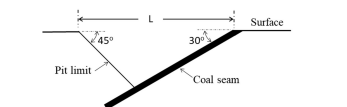
\includegraphics[width=0.4\columnwidth]{figs/pit.png}
  \caption{diagram}
  \label{fig:pit}
\end{figure}

\hfill\brak{GATE\ MN\ 2022}
\item A mine has a reserve of $150$ million tonne (Mt) and is designed for a maximum production capacity of $5$ Mt per year. In the first year the production is $2$ Mt and it increases by $20$\% each year. The reserve in Mt that remains at the end of $15$ years,is. (round off to two decimal places)

\hfill\brak{GATE\ MN\ 2022}
\item Information on Activity--Time duration of a project is provided below  
\begin{table}[H]
  \centering
  \caption{Match The Following}
  \input{Tables/Table10}
  \label{tab:table10}
\end{table}


\hfill\brak{GATE\ MN\ 2022}
\begin{center}
\Large\textbf{{END OF THE QUESTION PAPER}}
\end{center}
\end{enumerate}

\end{document}
